\documentclass[12pt, letterpaper]{article}

\usepackage{../../spreamble}
\usepackage{graphicx}

\title{CDA3101 - Buffer Overflow Lab}
\author{Ian Zou}

\begin{document}

\maketitle

\part*{Preface}

The lab template document wasn't working well for me; typing in the textboxes was a nightmare on every application I tried to the point I just decided to re-type everything into LaTeX. Sorry for the inconvenience, I hope this is not as bad to grade.

\part*{Task 1 - Compile \texttt{main.c}}

\subsection*{Describe what \texttt{main.c} does.}

\texttt{main.c} does some benign operations and then checks for input from the user.  However, this \texttt{get\_input} function uses \texttt{scanf} under the hood, which is very unsafe and prone to buffer overflow.

\subsection*{Show a screenshot of the compile command with your name somewhere in the screenshot.}

\textcolor{gray}{Note: I used the RISC-V cross-compiler and QEMU directly to run and debug it. Thus, the commands may look a little different, but rest assured everything works the same way.}

\medskip
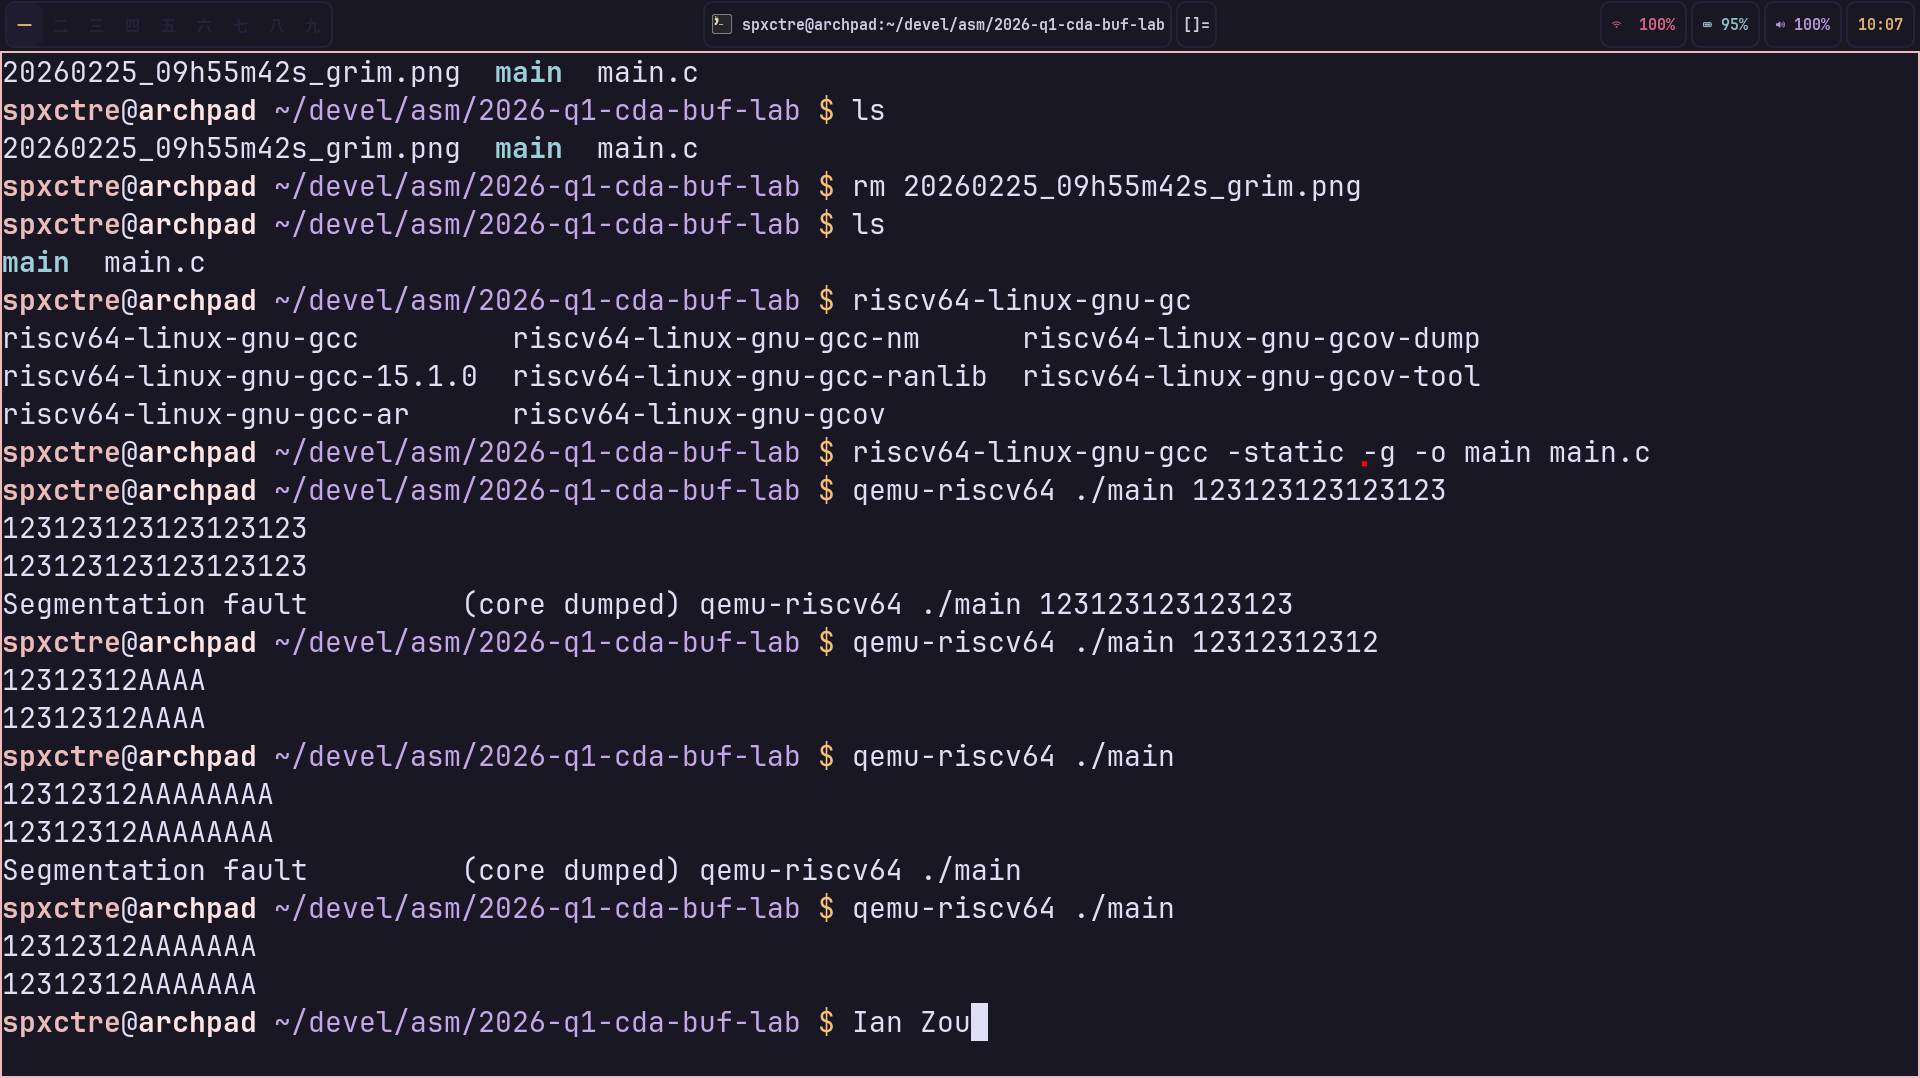
\includegraphics[width=\textwidth]{./screenshot.png}
\medskip

\part*{Task 2 - Run main from the deugger, without causing buffer overflow}

\subsection*{What do registers \texttt{ra} and \texttt{s0} represent?}

The \texttt{ra} register stores the return address of the function, which indicates where the function should jump to after the current function ends.
\medskip

\texttt{s0} is also known as the \texttt{fp} register, and call convention states that this is the register to save the frame pointer; which is needed to keep track of our current stack frame. When the current function ends, the \texttt{sp} stack pointer register will need to be collapsed to the frame pointer register in order to unload all the variables that were allocated on the stack during the execution of the current function, and thus these variables "leave scope."

\subsection*{Why are they placed on the stack?}

They are placed on the stack to be stored for later, since we are calling a function. When that function returns, the frame pointer would be collapsed to the stack pointer, and then the saved locals can be returned to the registers and allow the previous function to "function" as normal.


\subsection*{Run the following command: \texttt{disassemble get\_input}. Does \texttt{get\_input} save registers to the stack? Which ones?}

The \texttt{ra} and \texttt{s0} is saved onto the stack, since these registers may be overwritten by the called internal C function. This way, when this function returns we are able to restore these values into their corresponding registers and continue executing instructions from the returned-to function as normal.
\medskip

The reason we save the return address and frame pointer is because we need access to these values whenever the current values return. Since \texttt{ra} and \texttt{fp} may be overwritten by further function calls, we save them onto the stack. When our function returns, we are able to reload the frame pointer, collapse the stack pointer to the frame pointer, and jump back to the return address loaded into \texttt{ra} from the stack.

\subsection*{Table 1}

At the first line of \texttt{main}.

\begin{table}[h]
    \begin{center}
        \begin{tabular}{|c|c|}
            \hline
            \textbf{Register} & \textbf{Value} \\
            \hline
            \texttt{ra} & \texttt{0x10584} \\
            \hline
            \texttt{sp} & \texttt{0x7efc1f138600} \\
            \hline
            \texttt{s0} / \texttt{fp} & \texttt{0x7efc1f138620} \\
            \hline
    \end{tabular}
    \end{center}
\end{table}
\FloatBarrier

\subsection*{Table 2}

At the first line of \texttt{get\_input}.

\begin{table}[h]
    \begin{center}
        \begin{tabular}{|c|c|}
            \hline
            \textbf{Register} & \textbf{Value} \\
            \hline
            \texttt{ra} & \texttt{0x10506} \\
            \hline
            \texttt{sp} & \texttt{0x7f4f299385e0} \\
            \hline
            \texttt{s0} / \texttt{fp}  & \texttt{0x7f4f29938600} \\
            \hline
        \end{tabular}
    \end{center}
\end{table}
\FloatBarrier

\subsection*{Table 3}

Look at the contents of the stack with the following command: \texttt{x/4gx \$sp}.

\begin{table}[h]
    \begin{center}
        \begin{tabular}{|c|c|c|}
            \hline
            \textbf{Memory Address} & \textbf{Value} & \textbf{Value} \\
            \hline
            \texttt{0x7ff32b5d25e0} & \texttt{0x0000000700092188} & \texttt{0x0000000300000004} \\
            \hline
            \texttt{0x7ff32b5d25f0} & \texttt{0x00007ff32b5d2620} & \texttt{0x0000000000010506} \\
            \hline
        \end{tabular}
    \end{center}
\end{table}
\FloatBarrier

\subsection*{Using the values you entered in \textit{Table 2} and \textit{Table 3}, what are the addresses pointed to by A, B, and C in Figure 1?}

\begin{itemize}
    \item \texttt{A -> (0x7f4f299385e0)}
    \item \texttt{B -> (0x7efc1f138600)}
    \item \texttt{C -> (0x7efc1f138620)}
\end{itemize}

\subsection*{Table 4}

I typed in \texttt{12345678} and observed the values placed on the stack with the command \texttt{x/6gx \$sp}.

\begin{table}[h]
    \begin{center}
        \begin{tabular}{|c|c|c|}
            \hline
            \textbf{Memory Address} & \textbf{Value} & \textbf{Value} \\
            \hline
            \texttt{0x7ff32b5d25e0} & \texttt{0x0000000700092188} & \textcolor{red}{\texttt{0x3837363534333231}} \\
            \hline
            \texttt{0x7ff32b5d25f0} & \texttt{0x00007ff32b5d2600} & \texttt{0x0000000000010506} \\
            \hline
            \texttt{0x7ff32b5d2600} & \texttt{0x00000000000003e8} & \texttt{0x0000000700000002} \\
            \hline
        \end{tabular}
    \end{center}
\end{table}
\FloatBarrier

\part*{Task 3 - Run \texttt{main} from debugger, causing buffer overflow}

\subsection*{Table 5}

Typing in a string of 18 characters (\texttt{123456789012345678}) and observe the stack with \texttt{x/6gx \$sp}.

\begin{table}[h]
    \begin{center}
        \begin{tabular}{|c|c|c|}
            \hline
            \textbf{Memory Address} & \textbf{Value} & \textbf{Value} \\
            \texttt{0x7f89f64915e0} & \texttt{0x0000000700092188} & \texttt{0x3837363534333231} \\
            \texttt{0x7f89f64915f0} & \texttt{0x3635343332313039} & \texttt{0x0000000000003837} \\
            \texttt{0x7f89f6491600} & \texttt{0x00000000000003e8} & \texttt{0x0000000700000002} \\
            \hline
        \end{tabular}
    \end{center}
\end{table}
\FloatBarrier

\subsection*{What has happened to our stack frame for main?}

Our stack frame (and even our return address, it seems) have been overwritten by our buffer overflow. If only there was a way to buffer overflow with a payload that overwrites the return address into a function of our choice...

\subsection*{Type \texttt{n} until you see a message. Why did this happen?}

I used \texttt{c} to continue instead and got the message: "\texttt{Program received signal SIGSEGV, Segmentation fault.}" This segmentation fault occurs because we wrote past the bounds of our memory and corrupted the return address, and attempting to jump to a corrupt return address would fail and thus is why we got a segmentation fault.

\subsection*{Table 6}

Use \texttt{i r} again to to list out the information on all of the current registers.

\begin{table}[h]
    \begin{center}
        \begin{tabular}{|c|c|}
            \textbf{Register} & \textbf{Value} \\
            \texttt{ra} & \texttt{0x3837} \\
            \texttt{sp} & \texttt{0x7f89f6491600} \\
            \texttt{s0} / \texttt{fp} & \texttt{0x3635343332313039} \\
        \end{tabular}
    \end{center}
\end{table}

\subsection*{What happened to our \texttt{ra} and \texttt{s0} values?}

Our buffer overflow previously overwrote the stack frame and return address when it was stored on the stack, and now these values have been reloaded into the registers.

\part*{Task 4 - Record address for \texttt{arbitrary\_code} to function}

\subsection*{What is the address in memory of the first line of the \texttt{arbitrary\_code} function?}

By using \texttt{diassemble arbitrary\_code}, I was able to get the address as \texttt{0x10466}.

\part*{Task 5 - Run main from command line, overflow the buffer}

\subsection*{What happens when you input a string of 20 characters with no spaces?}

It prints what I inputted and then segmentation faults.

\medskip
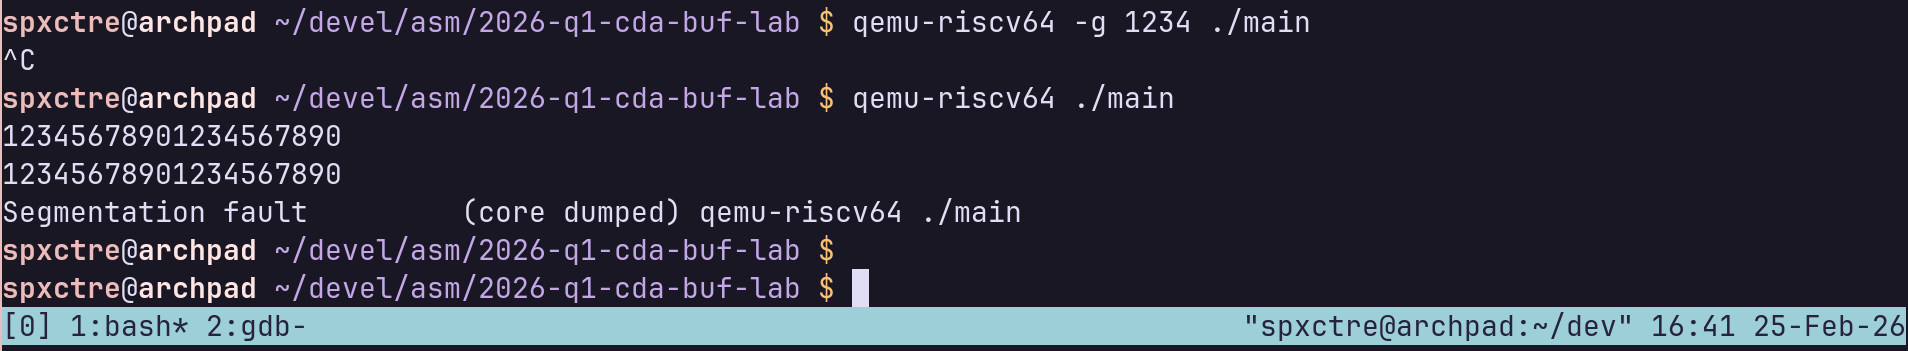
\includegraphics[width=\textwidth]{./task05_screenshot.png}
\medskip

\part*{Task 6 - Run \texttt{main} from command line, craft input to main to execute \texttt{arbitrary\_code} function}

\subsection*{What is ASLR?}

ASLR, or address space layout randomization, is a technique many operating systems and computers employ to prevent memory exploitation and corruption vulnerabilities. What ASLR does is that it randomly rearranges the address space positions of key data areas of a process.

\subsection*{Why do we need to turn off ASLR to make \texttt{arbitrary\_code} to run?}

We need to be able to exploit the return address consistently by replacing the return address with the address of \texttt{arbitrary\_code}. ASLR could play a part in making this unpredictable; for the purposes of our education we will turn off ASLR to demonstrate this buffer overflow vulnerability.

\subsection*{What happens?}

So I used \texttt{echo -e "ABCDEFGHIJKLMNOP\\x66\\x04\\x01" | qemu-riscv64 ./main} and got the buffer overflow to work. The program started spamming "\textit{Now you know I should not be seen ! But I am. Don't believe me just watch}" over and over again.

\part*{Task 7 - Turn ASLR back on}

\subsection*{What happens?}

So after typing in the specified commands, it printed a bunch of characters after the alphabet and then segmentatoin faulted as it did when the buffer overflowed but without a payload of the address of the \texttt{arbitrary\_code}.

\part*{Task 8 - Fix the vulnerability}

\subsection*{What happens?}
\texttt{fgets} ensures that only the specified length of characters is read in from \texttt{stdin}, thereby removing the possibility of a buffer overflow. Moreover, it makes sure to null terminate the buffer so that we know for a fact when this string ends. Therefore, when we input a value that is greater than 8 characters, it will truncate our input to 7 characters, replacing the 8th character with the null terminator.

\medskip
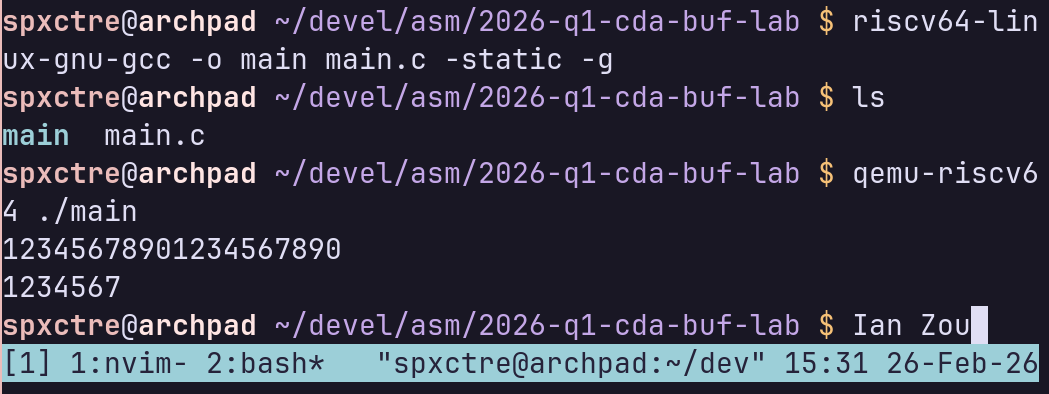
\includegraphics[width=\textwidth]{./task07-screenshot.png}
\medskip

\part*{Task 9 - Real-world application}

\subsection*{Research a CVE}

\begin{itemize}
    \item \textbf{CVE Number}: CVE-2025-8030
    \item \textbf{Name of Vulnerability}: Potential user-assisted code execution in "Copy as cURL" command
    \item \textbf{Affected software}: Firefox, Thunderbird
    \item \textbf{Reported From}: \texttt{https://bugzilla.mozilla.org/show\_bug.cgi?id=1968414}
    \item \textbf{Description}: Insufficient escaping in the “Copy as cURL” feature could potentially be used to trick a user into executing unexpected code. This vulnerability affects Firefox < 141, Firefox ESR < 128.13, Firefox ESR < 140.1, Thunderbird < 141, Thunderbird < 128.13, and Thunderbird < 140.1.

\end{itemize}

\subsection*{Why do you think there are still vulnerabilities like this?}

People all around the world believe they can write safe C, and then use unsafe functions that have the chance to buffer overflow if used incorrectly. Moreover, there are many libraries that call upon the (potentially) unsafe C functions that are kept for historic purposes, unbeknowst to the vulnerabilities that they have. Combined with increase use of artificial intelligence and cognitive debt in programming in the 21st century, all of these factors lead to these security vulnerabilities still existing nowadays.

\end{document}

